\documentclass{article}

\usepackage[dblblindworkshop]{neurips_2026}
\workshoptitle{Interpretability as a Science}

\usepackage[utf8]{inputenc}
\usepackage[T1]{fontenc}
\usepackage{hyperref}
\usepackage{url}
\usepackage{booktabs}
\usepackage{amsfonts}
\usepackage{amsmath}
\usepackage{amssymb}
\usepackage{microtype}
\usepackage{graphicx}
\usepackage{xcolor}

\title{Circular axes and photo-present artifacts:\\
a measurement audit of visual affect in vision-language models}

\author{Anonymous Author(s)}

\begin{document}

\maketitle

\begin{abstract}
A residual-stream contrast is sometimes treated as a measurement of visual affect, and a change in model answers is then read as evidence that the construct is causal. That inference can fail. We report Gemma-4 experiments on EMOTIC, a frozen mechanism artifact, and writeup numbers from a concurrent Gemma-3 / OASIS program. An affect axis built from photographs makes $|\Delta_{\mathrm{img}}|/|\Delta_{\mathrm{txt}}|$ reconstruct the defining contrast: the recorded $\mathrm{ratio}_a=1.591$ is a metric on that construction, and it is not a ranking of how affective images are relative to text. On harmful prompts, negative and neutral photos leave refusal at ceiling (Gemma-4-E4B-it Grok refuse $0.99$ to $1.00$, $n=100$; Gemma-3-12B writeup first-token refuse $0.99$ across valences). A locked battery on Gemma-4-E4B-it and Gemma-4-12B-it finds that a photo raises full-answer refuse on benign XSTest items. Named-emotion ladders, ultimatum unfair-reject, and frozen $a_\perp$ mediation do not hold. Neutral photos fall in the photo cluster. Photo presence is a safety-context artifact. A visual-affect claim needs a cross-built axis, a locked scorer, and alternatives that fail. A large projection on the contrast used to define the axis does not suffice.
\end{abstract}

\section{Introduction}
\label{sec:intro}

Difference-of-means on last-token residuals yields a unit vector that can be projected, steered, and plotted. Calling that vector affect, refusal, or jailbreak is a measurement claim: the score should still track the intended construct if the defining contrast were built another way \citep{cronbach1955construct,messick1995validity,borsboom2004concept}. Adjacent fields already ask what is measured, what would falsify it, and which artifacts produce the same number \citep{doshi2017towards,lipton2018mythos}.

Text-only models have a valence-arousal subspace that can move refusal \citep{sun2026valence}. Refusal can be a single residual direction $r$ \citep{arditi2024refusal}. If a sad or frightening photograph loaded that subspace, a large image $\Delta$ on an affect axis would be expected, as would emotion-specific changes on economic and safety tasks, and a drop in refuse on harmful asks. We tested those predictions on Gemma-4 \citep{gemmateam2026gemma4} with EMOTIC people-in-context labels \citep{kosti2017emotion,kosti2019emotic}, and we compare the results to writeup numbers from a concurrent Gemma-3 / OASIS program \citep{gemmateam2025gemma3,kurdi2017oasis}. The two stacks are not pooled.

When $a$ is built from negative versus neutral photographs under a DESCRIBE prompt, $|\Delta_{\mathrm{img}}|/|\Delta_{\mathrm{txt}}|$ on that axis measures how well the defining contrast reconstructs itself. An earlier full-tier run recorded $\mathrm{ratio}_a=1.591$ and labeled it \texttt{INVERTED}. We withdraw that label as a modality ranking (Section~\ref{sec:circular}).

Emotional photographs do not jailbreak under the recorded protocols (Section~\ref{sec:null}). A later frozen joint-axis run replaces the withdrawn ranking with \texttt{MAGNITUDE\_GAP}: photos move a combined $a_\perp$ under DESCRIBE, that $\Delta$ shrinks under harmful asks, and restoring it does not drop refuse (Section~\ref{sec:v3}).

A confirmatory battery wrote \texttt{LOCK.json} before scoring. On official XSTest safe items \citep{rottger2024xstest}, attaching an EMOTIC photo raises full-answer refuse versus no image on both Gemma-4-E4B-it (encoder) and Gemma-4-12B-it (unified). Neutral sits in the photo cluster. Emotion-specific ladders fail. Ultimatum unfair-reject is a floor. Frozen $a_\perp$ mediation was missing on the pod (Section~\ref{sec:battery}).

Photographs do not induce emotion in the model on this evidence. Several common interpretability moves fail construct checks. The remaining behavioral fact is extra caution when any photo is attached to a benign question that sounds sensitive.

\section{Related work}
\label{sec:related}

\paragraph{Refusal geometry.}
\citet{arditi2024refusal} extract $r$ as the mean last-token residual difference between harmful and harmless instructions. Adding scaled $+r$ to harmless prompts induces refuse; erasing $r$ can remove it. Orthogonalizing a second concept against $r$ does not make that concept causally independent of refusal \citep{wollschlager2025geometry}. Interventions follow activation addition \citep{turner2023activation,rimsky2024steering}.

\paragraph{Affect as a control axis.}
\citet{sun2026valence} recover a 2D valence-arousal subspace in text-only models and show that steering it modulates refusal and sycophancy. \citet{zhou2024alignment} argue that alignment ties mid-layer negative emotion to refuse tokens. Those papers motivate a VLM test. They do not show that pixels load the same gate.

\paragraph{Image corpora.}
EMOTIC labels the emotion of a depicted person in context \citep{kosti2017emotion,kosti2019emotic}. OASIS is a viewer-normed valence/arousal set \citep{kurdi2017oasis}. A depicted-anger photograph is not a high-arousal viewer rating. We treat corpus as a science factor and do not pool.

\paragraph{Behavior batteries.}
Over-refusal on safe items that sound sensitive is the XSTest problem \citep{rottger2024xstest}. Economic items follow dictator/ultimatum conventions \citep{forsythe1994fairness} and Kirby-style now-versus-later choices \citep{kirby2000discounting}. Perez-style sycophancy \citep{perez2022discovering} and TruthfulQA \citep{lin2022truthfulqa} appear only as exploratory or aborted endpoints in our archive (Appendix~\ref{app:failed}).

\paragraph{Shared affect.}
A cross-modal test builds the axis on text and scores held-out images, or the reverse, with a caption control \citep{campbell1959convergent}. A concurrent text-trained pleasantness probe on Gemma-3-4B reported Spearman $\rho \approx 0.51$ against image valence on a full split ($n=7280$) and a unique-image residual after captions. That is a transfer measurement. It is not a residual $\Delta$ on an image-built DESCRIBE axis.

\section{Protocol}
\label{sec:protocol}

The audit uses three Gemma-4 artifacts and one teammate writeup. Effect sizes are not pooled across rows of Table~\ref{tab:stacks}.

\begin{table}[t]
\caption{Science stacks. Dtype, corpus, and axis construction are factors. Rows are not pooled.}
\label{tab:stacks}
\centering
\footnotesize
\begin{tabular}{@{}llll@{}}
\toprule
Item & Publish (image-only $a$) & Frozen mechanism v3 & Locked battery v2 \\
\midrule
Model & Gemma-4-E4B-it & Gemma-4-E4B-it & E4B-it and 12B-it \\
Vision & encoder & encoder & encoder vs unified \\
Dtype & nf4 & nf4 & bf16, no quant \\
Images & EMOTIC & EMOTIC & EMOTIC exclusive labels \\
Primary $a$ & image-only $a_\perp$ & joint $a_\perp$ & not scored (dirs missing) \\
Split & \texttt{ef2a7d2a84a803c7} & \texttt{1e8ea1c22144dd9d} & \texttt{1e8ea1c22144dd9d} \\
Lock before score & no & plan-locked & \texttt{LOCK.json} per cell \\
\bottomrule
\end{tabular}
\end{table}

\paragraph{Joint axis (frozen v3).}
Let $h_\ell(x)$ be the last prompt-token residual at layer $\ell$. Write $\mathrm{unit}(v)=v/\|v\|$.
\begin{align}
r &= \mathrm{unit}\!\left(\mathbb{E}[h(\mathrm{harmful})]-\mathbb{E}[h(\mathrm{harmless})]\right), \\
a_{\mathrm{img}} &= \mathrm{unit}\!\left(\mathbb{E}[h(\mathrm{DESCRIBE}{+}\mathrm{neg})]-\mathbb{E}[h(\mathrm{DESCRIBE}{+}\mathrm{neu})]\right), \\
a_{\mathrm{text}} &= \mathrm{unit}\!\left(\mathbb{E}[h(\mathrm{distress\ text})]-\mathbb{E}[h(\mathrm{neutral\ text})]\right), \\
a_\perp &= \mathrm{orth}_{\mathrm{span}}\!\left(\mathrm{unit}(a_{\mathrm{text}}+a_{\mathrm{img}}),\, r\right).
\end{align}
DESCRIBE is the string ``Describe what is happening in this image.'' Image-only $a_\perp$ is a named variant. Orthogonalization is QR on the span. The layer window for $L=42$ is $[10,25)$; for $L=48$, $[12,28)$. Equivalent form: $[\lfloor 0.25L\rfloor, \lfloor 0.60L\rfloor)$. Steer on gate layers is $\mathrm{resid}_\ell \leftarrow \mathrm{resid}_\ell + \alpha\,\|\mathrm{resid}_\ell\|\,\widehat{d}_\ell$. Shared code pins $\alpha=0.008$ as the default dose. The frozen v3 sweep uses the coarser grid $\{0.1,0.25,0.4,0.6,0.9\}$ and reports ceilings at $0.4$.

\paragraph{Locked battery rules (v2).}
Each cell writes \texttt{LOCK.json} (script hash, split, seed, image ids) before the first score. The scorer refuses if the lock is missing or hashes drifted. Thinking mode is off. Chat order is $[\mathrm{image},\,\mathrm{text}]$. The task prompt is not preceded by DESCRIBE. Neutral is the exclusive-label remainder: none of fear, anger, sadness, excitement, happiness, or peace. Neutral is not Peace. EMOTIC and OASIS are not pooled. E4B versus 12B is encoder versus unified; it is not a scale comparison. Full-answer refuse on XSTest does not treat a bare ``I'' ($|\mathrm{token}|\le 2$) as refuse. First-token ``I'', ``As'', and ``Of'' go in a secondary \texttt{ambiguous\_v1} bin. An earlier exploratory run had counted ``I'' as refuse.

\paragraph{Closed endpoints.}
An EmoBank valence-arousal sycophancy confirmatory aborted on official splits ($r_V=0.446$, $r_A=0.236$ against a $r\ge 0.7$ gate). Local color-square dry runs are invalid. Frozen v3 JSON is read-only.

\section{Circularity}
\label{sec:circular}

Construct validity asks whether a score still means the same thing under a different operationalization \citep{messick1995validity}. For residual directions, the operationalization is the contrast.

A full-tier publish run on Gemma-4-E4B-it (nf4, Tesla T4, EMOTIC, $N_\Delta=40$) built $a$ from images under DESCRIBE and recorded $\mathrm{ratio}_a=|\Delta_{\mathrm{img}}|/|\Delta_{\mathrm{txt}}|=1.591$ ($\delta_{\mathrm{txt},a}=3.401$, $\delta_{\mathrm{img},a}=5.411$), labeled \texttt{INVERTED}. The same run's OOD residual-norm check passed (science/ref $\approx 1.003$). Unit-norming left $\mathrm{ratio}_a=1.390$, still inverted. Those checks rule out color-square norm inflation. They leave construction bias in place: the numerator is the defining contrast.

Table~\ref{tab:three} records three numbers that are not interchangeable.

\begin{table}[t]
\caption{Three affect/refusal numbers. Each row is a different estimand.}
\label{tab:three}
\centering
\footnotesize
\begin{tabular}{@{}p{0.20\linewidth}p{0.44\linewidth}p{0.26\linewidth}@{}}
\toprule
Name & Definition & Recorded value \\
\midrule
Gemma-3 writeup $100\times$ & Harmful-prompt image $\Delta$ on $a_\perp$ vs.\ jailbreak steer & $\sim$11 to $22$ vs.\ $\sim$2200 \\
v3 suppression & Bootstrap median of $\Delta_{\mathrm{harm}}/\Delta_{\mathrm{DESCRIBE}}$ on joint $a_\perp$ & $0.107$, 95\% CI $[0.079,0.130]$ \\
Publish $\mathrm{ratio}_a$ & $|\Delta_{\mathrm{img}}|/|\Delta_{\mathrm{txt}}|$ on image-built $a_\perp$ & $1.591$ (construction-biased) \\
\bottomrule
\end{tabular}
\end{table}

We withdraw the claim that photographs are intrinsically more emotional than text. The number that remains is that an image-defined contrast reconstructs itself more cleanly than a mismatched text string. v3 rebuilt the axis as $\mathrm{orth}(\mathrm{unit}(a_{\mathrm{text}}+a_{\mathrm{img}}),r)$ and used a text bank of 64 distress and 64 neutral items. Diagnostic splits on that file still show image-built $\Delta_{\mathrm{DESCRIBE}}=5.396$ versus text-built $0.146$. That split is expected under the construction. It is not a second \texttt{INVERTED} headline.

\section{Harmful prompts}
\label{sec:null}

A jailbreak account of visual affect predicts that negative photos lower refuse on harmful instructions \citep{zou2023universal}. That drop is absent on both stacks we can cite.

On frozen v3 (Gemma-4-E4B-it, A100, split \texttt{1e8ea1c22144dd9d}, $N_{\mathrm{BEH}}=100$, $N_{\mathrm{BORDER}}=80$), first-token refuse on harmful prompts is $0.99$ (no image), $1.00$ (negative), and $1.00$ (neutral). Grok refuse is $0.99$, $0.99$, and $1.00$. Borderline cells are $1.00$ first-token and $0.9875$ Grok in every image arm. Gates B1 and B2 hold. $\texttt{images\_jailbreak}=\texttt{false}$. The earlier publish Grok table ($n=100$, fallback $0\%$) is $1.00$ / $1.00$ / $0.98$ (no image / negative / neutral).

A concurrent Gemma-3-12B / OASIS writeup reports first-token refuse $0.99$ for neu, neg, and pos image arms and $0.99$ with no image. Tensors from that run were not imported. We cite the writeup as a second protocol, not a replication of weights. Early incomplete EMOTIC downloads on that program (about $184$ images, including a one-image negative set) are retired.

The null is restricted to harmful-prompt refuse. Pixels can still move residual scores (Section~\ref{sec:v3}). Photos can still change answers on benign items (Section~\ref{sec:battery}).

\section{Locked battery}
\label{sec:battery}

Battery v2 ran on one RTX PRO 6000 (96\,GB) at locked tier \texttt{budget3h}: $n_{\mathrm{safe}}=80$ XSTest items, $4$ images per emotion arm, seed $2$, exclusive EMOTIC labels, split \texttt{1e8ea1c22144dd9d}. Twelve EMOTIC cells completed (two models $\times$ six tests). OASIS cells were planned and are not on disk.

\subsection{Over-refusal on safe items}
\label{sec:exp09}

The primary dependent variable is full-answer refuse on official XSTest safe items. Figure~\ref{fig:exp09} and Table~\ref{tab:exp09} report the locked result.

\begin{figure}[t]
\centering
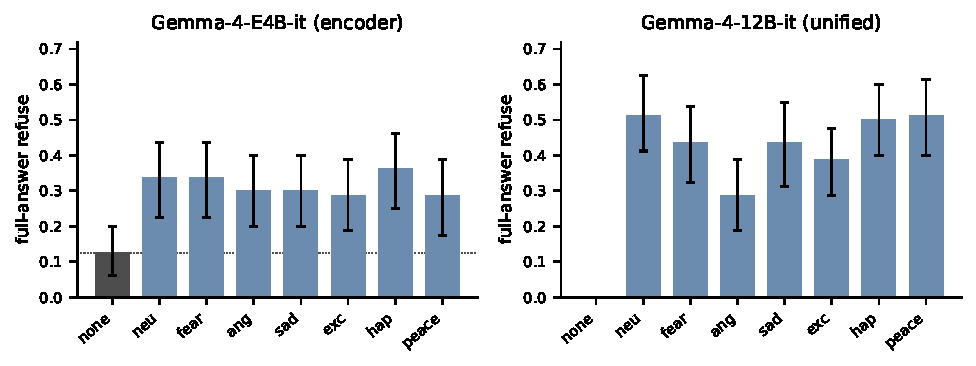
\includegraphics[width=\linewidth]{figures/fig_exp09.pdf}
\caption{Locked exp09: full-answer refuse on $n=80$ XSTest safe items. Error bars are the recorded cluster intervals. Neutral (neu) is a photo arm. Peace is a named emotion, distinct from Neutral.}
\label{fig:exp09}
\end{figure}

\begin{table}[t]
\caption{Locked exp09 refuse rates (EMOTIC). Intervals are those stored in the result JSON. $\Delta$ is versus no-image.}
\label{tab:exp09}
\centering
\footnotesize
\begin{tabular}{@{}lcccc@{}}
\toprule
Arm & E4B rate & E4B 95\% CI & 12B rate & 12B 95\% CI \\
\midrule
no image & $0.125$ & $[0.062,0.200]$ & $0.000$ & $[0.000,0.000]$ \\
neutral & $0.338$ & $[0.225,0.438]$ & $0.512$ & $[0.412,0.625]$ \\
fear & $0.338$ & $[0.225,0.438]$ & $0.438$ & $[0.325,0.538]$ \\
anger & $0.300$ & $[0.200,0.400]$ & $0.288$ & $[0.188,0.388]$ \\
sadness & $0.300$ & $[0.200,0.400]$ & $0.438$ & $[0.312,0.550]$ \\
excitement & $0.288$ & $[0.188,0.388]$ & $0.388$ & $[0.288,0.475]$ \\
happiness & $0.362$ & $[0.250,0.462]$ & $0.500$ & $[0.400,0.600]$ \\
peace & $0.288$ & $[0.175,0.388]$ & $0.512$ & $[0.400,0.613]$ \\
\bottomrule
\end{tabular}
\end{table}

On E4B, no-image refuse is $0.125$. Photo arms sit at $0.288$ to $0.362$. Neutral and fear match at $0.338$. Happiness is highest at $0.362$. The Neutral, fear, and happiness intervals miss the no-image interval. Several other photo arms touch or overlap $0.200$. Photo arms overlap each other. On 12B, no-image refuse is $0.000$ and every photo interval starts at or above $0.188$. Neutral equals Peace at $0.512$. Anger ($0.288$) sits below Neutral ($0.512$); those intervals do not overlap. The anger gap has the opposite sign from a distress account.

First-token refuse is near zero. The v1-style ``I'' mass lands in \texttt{ambiguous\_v1} (E4B: $18$ no-image versus $32$ to $37$ photo, of $88$ rows including $8$ unsafe). The photo-present jump remains after the scorer stops treating ``I'' as refuse. An earlier unlocked E4B run ($n=250$, first-token, ``I'' counted as refuse) already showed the same direction (no-image $0.656$, photo arms $0.908$ to $0.944$, Neutral highest). Absolute rates are not comparable across scorers.

\subsection{Games, waiting, and cross-modal}
\label{sec:other}

Table~\ref{tab:verdicts} summarizes the remaining locked EMOTIC cells.

\begin{table}[t]
\caption{Locked v2 EMOTIC verdicts. HOLDS means complete, required gates true, and the pre-specified contrast interval excludes zero (or arm intervals do not overlap).}
\label{tab:verdicts}
\centering
\footnotesize
\begin{tabular}{@{}lll@{}}
\toprule
Cell & Photo-present & Named emotion \\
\midrule
E4B exp09 refuse & HOLDS & NULL (arms overlap) \\
12B exp09 refuse & HOLDS & NULL (anger below Neutral) \\
E4B / 12B ultimatum reject & NULL (floor $0$) & NULL (floor $0$) \\
E4B dictator $0$ to $50$ & HOLDS ($0$ vs.\ $\approx 22$) & NULL ($7/8$ arms identical) \\
12B dictator $0$ to $50$ & NULL vs.\ no-image & some photo-vs-photo gaps \\
E4B $p(\mathrm{now})$ & partial & NULL vs.\ Neutral \\
12B $p(\mathrm{now})$ & NULL & NULL \\
E4B CROSS\_MODAL & n/a & pixels INCONCLUSIVE \\
12B CROSS\_MODAL & n/a & pixels DIVERGE vs.\ caption \\
exp10 / mech & n/a & \texttt{DIAGNOSTIC\_NOT\_V3} \\
\bottomrule
\end{tabular}
\end{table}

Ultimatum unfair-reject (80-20 and 90-10, $n=16$ per arm) is $0.0$ $[0.0,0.0]$ on both models and all eight arms. An exploratory v1 anger-reject contrast ($+0.073$, CI $[0.032,0.123]$) does not confirm; that run also had no-image reject $\approx 0.098$, close to anger. E4B dictator means are $0$ with no image and $18.75$ to $21.875$ with a photo; seven of eight photo arms are identical at $21.875$. 12B dictator intervals versus no-image overlap. Anger versus Peace separates, and anger still overlaps no-image.

Kirby $p(\mathrm{now})$ is a smoke grid ($n_{\mathrm{img}}=4$). E4B no-image is $0.50$ $[0.31,0.66]$ ($n=32$). Sadness and peace sit above that interval; several other photo arms overlap it. On 12B all arms overlap. There is no emotion-specific discount-rate ladder. Kirby $k$ is diagnostic only.

Cross-modal (anger versus Neutral, $n=16$ pairs): E4B headline \texttt{INCONCLUSIVE} (pixels not identifiable). 12B headline \texttt{CROSS\_MODAL\_DIVERGE}: pixels dictator $0.438$ $[0.125,0.688]$ identifiable, caption not. Label-only dictator is a text effect with opposite sign on 12B ($-1.0$). Six-way pixel expansion is $n=8$ without intervals.

\subsection{Failed emotion-specific predictions}
\label{sec:falsify}

A visual-affect account of these tasks predicted fear versus anger on risk and giving, anger raising unfair-reject, an impatience order by emotion, Neutral matching no-image or Peace, and pixel effects that captions copy. The locked battery fails the unfair-reject, impatience, Neutral, and emotion-specific risk/giving predictions. Photo presence remains: attaching an EMOTIC still changes some answers, most cleanly as extra caution on XSTest-safe items. That is a measurement of a vision-conditioned safety policy.

\section{Mechanism}
\label{sec:v3}

Frozen v3 is the only locked mechanism artifact. It uses the joint $a_\perp$ of Section~\ref{sec:protocol}. $r$ is competent: harmless first-token refuse $0.083\to 1.0$. An independent jailbreak direction $j$ from natural refuse/comply terciles has $|\cos(j,r)|=0.247$ (status \texttt{INDEPENDENT}). Geometry: $|\cos(a_{\mathrm{text}},r)|=0.169$, $|\cos(a_{\mathrm{img}},r)|=0.135$, $|\cos(a_{\mathrm{text}},a_{\mathrm{img}})|=0.098$. OOD residual-norm PASS (ratio $1.002$).

Under DESCRIBE, combined $a_\perp$ moves: $\Delta_{\mathrm{DESCRIBE}}=3.664$, whitened null $p=0$, $n_\Delta=64$, correlational M1 true. Under harmful prompts, $\Delta_{\mathrm{harm}}=0.389$. Suppression ratio $0.107$, 95\% CI $[0.079,0.130]$ from $1{,}000$ paired-image bootstrap medians. Figure~\ref{fig:layers} shows the layer curves. DESCRIBE $\Delta$ grows through the gate and beyond; harmful $\Delta$ stays small. $R_{\mathrm{affect}}=0.0050$ compares the natural harmful-context move to the v3 affect-steering ceiling at $\alpha=0.4$. That is a reachability ratio, distinct from $\mathrm{ratio}_a$ and from the Gemma-3 writeup's $\sim 100\times$.

\begin{figure}[t]
\centering
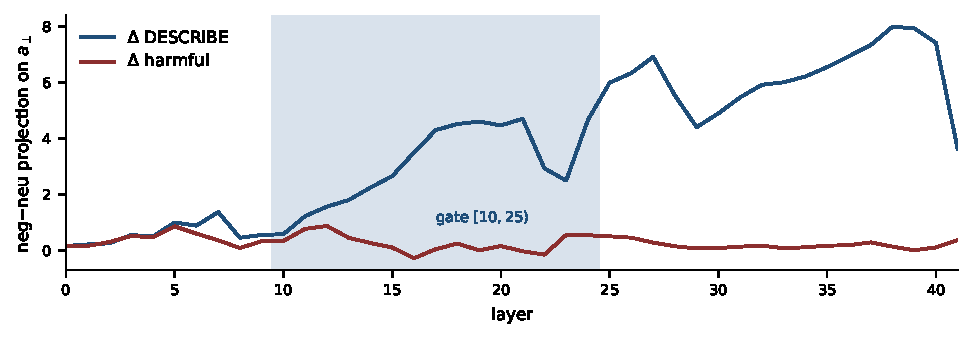
\includegraphics[width=\linewidth]{figures/fig_layers.pdf}
\caption{Frozen v3 layer-wise neg$-$neu projection on joint $a_\perp$. The shaded band is the locked gate $[10,25)$ for $L=42$. Photos move the axis under DESCRIBE. The same contrast is small under harmful asks.}
\label{fig:layers}
\end{figure}

Causal restore (C1) fails: $\mathrm{drop}_{\mathrm{clean}}=1.68 < \mathrm{drop}_{\mathrm{rand}}=7.56$. Refuse-rate drop under clean restore is $0.0$. $\texttt{M1\_causal}=\texttt{false}$. Images miss $j$ ($s_{j,\mathrm{neg}}=4.275$ versus $s_{j,\mathrm{neu}}=4.451$). Caption $\Delta$ under DESCRIBE is $1.533$; the file marks caption as not vision-specific. The file's one-line summary is the claim we keep: photos move the emotion direction under DESCRIBE, and under harmful asks the push is small next to the steer that jailbreaks.

Battery v2 exp10 and mech cells completed with $\texttt{dirs\_status}=\texttt{DIAGNOSTIC\_NOT\_V3}$, $\texttt{dirs\_path}=\texttt{null}$, $\texttt{ab}=\texttt{null}$, and $\texttt{a\_perp\_present}=\texttt{false}$. E4B exp10 records a paired risk shift $c=0.114$ $[0.035,0.209]$ without an $ab$ path; $\texttt{frozen\_ok}=\texttt{false}$. 12B exp10 has $\texttt{fc\_mass}=0.532<0.8$ (endpoint invalid) and a $c$ interval that includes zero. Those cells are not mediation.

The Gemma-3-12B writeup reports a coherent $-a_\perp$ gate (base refuse $0.99$, affect-steer $0.04$, random $0.99$ at $\alpha=0.008$) and $r$-restore ($0.25\to 1.00$). We did not import those tensors. Gemma-4 v3 does not reproduce that causal gate. The stacks differ in model family, dtype, corpus, and axis. The shared behavioral fact is the image-null on harmful refuse.

\section{Criteria}
\label{sec:discuss}

\citet{lipton2018mythos} noted that interpretability language can outrun the tests that would distinguish a mechanism from a story. For visual affect we use four checks. This archive fails each of them in at least one recorded run.

\begin{enumerate}
\item \textbf{Construction.} State how the axis was built before ranking modalities. Image-built $\Delta_{\mathrm{img}}$ is not a transfer result. Cross-build (text $\to$ image, or image $\to$ text) with a caption semipartial is the Campbell--Fiske move \citep{campbell1959convergent}.
\item \textbf{Scoring.} A first-token lexicon that includes ``I'' scores hedging as refuse. Lock the scorer and report the secondary bin the lock rejected.
\item \textbf{Controls.} Neutral photographs, Peace photographs, and no image are three arms. If Neutral tracks other photos, the construct is not depicted emotion.
\item \textbf{Causal sufficiency.} A correlational $\Delta$ under DESCRIBE is not mediation \citep{baron1986moderator}. Restore or ablate at image scale under the task prompt. v3 C1 is the failed version of that test.
\end{enumerate}

Photo-present extra caution is a real interpretability object. Chat VLMs see images in contexts where refusal and hedging are common, so the same object is also a plausible training artifact. Reading that policy as fear or sadness is a construct error. The locked battery is a negative result on the emotion-specific hypotheses that would have supported that reading.

\section{Limitations}
\label{sec:limitations}

nf4 (publish, v3) versus bf16 (battery v2) is an unquantified confound. E4B versus 12B mixes architecture with size. EMOTIC negative exclusive pools are small relative to Neutral. Battery v2 used four images per arm and $80$ safe items; intervals are wide. OASIS v2 scores are missing. Frozen $a_\perp$ / $r$ tensors are not in the repository (\texttt{*.pt} was never checked in; v2 mech could not score $a_\perp$). Gemma-3 writeup numbers are not a local JSON. Direction rebuilds planned at three seeds were not done. The sycophancy confirmatory aborted. Results are instruction-tuned Gemma, not a survey of deployed systems. Orthogonalizing to $r$ does not make $a$ refusal-independent \citep{wollschlager2025geometry}.

\section{Broader impacts}
\label{sec:impacts}

If the photo-present extra-caution effect is real, attaching an irrelevant photograph to a benign question can raise refuse. That can hide capability and can look like safety. If the harmful-prompt image-null is real, emotional photographs are not an input-space jailbreak under these protocols. White-box affect steering remains an exposure on the Gemma-3 writeup stack. We do not package an attack tool. Harmful completions were generated only for Grok classification on named Gemma-4 behavioral arms. The JSON artifacts retain aggregate rates, not completion text. Image sets are existing public corpora.

\section{Conclusion}
\label{sec:conclusion}

Visual-affect interpretability fails standard measurement checks when the axis is the contrast, Neutral is treated as Peace, and ``I'' is treated as refuse. After those checks, two facts remain. Emotional photographs do not lower refuse on harmful prompts. On a locked Gemma-4 battery, a photograph raises refuse on benign XSTest items, and named emotion does not explain the rest of the board. The supported reading is a photo-present artifact plus a magnitude gap.

\small
\bibliographystyle{plainnat}
\bibliography{references}

\appendix

\section{Exploratory v1 board}
\label{app:v1}

Battery v1 (Gemma-4-E4B-it, nf4, 8$\times$A100, split \texttt{1e8ea1c22144dd9d}) finished ten experiments without pre-score \texttt{LOCK.json}. Frozen v3 was not overwritten. Labels below are scientific labels, not run-status labels.

\begin{table}[h]
\caption{Exploratory v1. HOLDS means a contrast interval excluded zero and the endpoint parsed. The campaign is not confirmatory.}
\label{tab:v1}
\centering
\footnotesize
\begin{tabular}{@{}llp{0.52\linewidth}@{}}
\toprule
ID & Label & One-line result \\
\midrule
01 & NULL & Fear vs.\ anger $p(\mathrm{risky})$ $\Delta=-0.092$, CI $[-0.50,0.30]$ \\
02 & NULL & No exp01 effect to attribute to scene match \\
03 & exploratory & Pixel dictator $n=8$, $\Delta\approx-0.98$; smoke \\
04 & NULL & Perez vs.\ Neutral $\Delta=-0.065$, CI includes $0$ \\
05 & exploratory & Anger reject $+0.073$; no-image reject $\approx$ anger \\
06 & photo vs.\ none & $p(\mathrm{now})$ $0.36$ vs.\ photo $0.44$ to $0.54$; no $k$ ladder \\
07 & NULL & Trivia equivalence inconclusive; no affect-collapse \\
08 & NULL & EMOTIC vs.\ OASIS smoke: both-null; do not pool \\
09 & HOLDS & First-token refuse $0.656\to 0.91$ to $0.94$; Neutral highest \\
10 & diagnostic & Dirs not v3; dictator mass $0.27$; risk $ab$ correlational \\
\bottomrule
\end{tabular}
\end{table}

v2 confirmed the photo-present reading of exp09 under a stricter scorer. It did not confirm v1 anger-reject or a frozen mediation path.

\section{Hashes and compute}
\label{app:hash}

Publish prereg \path{3111c3af7f7b12656cb0792bea4a21b4302a0c42}.
Publish split \path{ef2a7d2a84a803c7}.
v3 / battery split \path{1e8ea1c22144dd9d}.
v2 script sha256 \path{58cb87976fe09225e3cd7da6e4a808b1ac9797ee8e6ca975407545e96e981856}.
XSTest pin (LF-normalized) \path{11783fb294ed017473ee53c207d71f2161c7672c8d0b037501e78387f801cb5a}.
v2 exp09 image-id sha256 \path{20bd27f254e2fc507e1f16244701cb97b7f8fcfc2af19a980468feb9bed76965}.

Compute recorded: publish pipeline Tesla T4 $\sim$8942\,s; v3 A100-SXM4-40GB $6740.5$\,s; battery v2 one RTX PRO 6000 96\,GB, locked 3-hour budget. Gemma-3 writeup GPU and wall time are not recorded. Failed sycophancy smokes and v1 A100 nights are extra project compute.

\section{Aborted and invalid endpoints}
\label{app:failed}

EmoBank-VA sycophancy, official splits: $r_V=0.446$, $r_A=0.236$, \texttt{ENDPOINT\_INVALID}. Earlier smokes: Likert digit mass $0.181$; truncated $N=64$ bank; $r_A=-0.019$. Local RTX 3050 color squares: $\mathrm{ratio}_a\sim 192$, invalid. Gemma-3-4B fallback smoke is not primary. v1 exp05 run1/run2 letter mass $<0.8$: do not cite. v2 12B exp10 letter mass $0.532$: do not cite $c$.

\newpage
% NeurIPS 2026 paper checklist. Do not modify the questions.

\section*{NeurIPS Paper Checklist}

\begin{enumerate}

\item {\bf Claims}
\item[] Question: Do the main claims made in the abstract and introduction accurately reflect the paper's contributions and scope?
\item[] Answer: \answerYes{}
\item[] Justification: Abstract and Section~\ref{sec:intro} state three surviving claims (circularity of image-built $\mathrm{ratio}_a$, harmful-prompt refuse ceiling, locked photo-present over-refusal) and withdraw emotion-specific and causal-mediation headlines. We do not claim that photographs induce emotion.
\item[] Guidelines:
\begin{itemize}
\item The answer \answerNA{} means that the abstract and introduction do not include the claims made in the paper.
\item The abstract and/or introduction should clearly state the claims made, including the contributions made in the paper and important assumptions and limitations. A \answerNo{} or \answerNA{} answer to this question will not be perceived well by the reviewers.
\item The claims made should match theoretical and experimental results, and reflect how much the results can be expected to generalize to other settings.
\item It is fine to include aspirational goals as motivation as long as it is clear that those goals are not attained by the paper.
\end{itemize}

\item {\bf Limitations}
\item[] Question: Does the paper discuss the limitations of the work performed by the authors?
\item[] Answer: \answerYes{}
\item[] Justification: Section~\ref{sec:limitations} and Appendix~\ref{app:failed} cover quantization, architecture mix, missing OASIS v2, missing frozen tensors, single-seed directions, aborted sycophancy, and writeup-only Gemma-3 numbers.
\item[] Guidelines:
\begin{itemize}
\item The answer \answerNA{} means that the paper has no limitation while the answer \answerNo{} means that the paper has limitations, but those are not discussed in the paper.
\item The authors are encouraged to create a separate ``Limitations'' section in their paper.
\item The authors should point out any strong assumptions and how robust the results are to violations of these assumptions.
\item The authors should reflect on the scope of the claims made, e.g., if the approach was only tested on a few datasets or with a few runs.
\item Reviewers will be specifically instructed to not penalize honesty concerning limitations.
\end{itemize}

\item {\bf Theory assumptions and proofs}
\item[] Question: For each theoretical result, does the paper provide the full set of assumptions and a complete (and correct) proof?
\item[] Answer: \answerNA{}
\item[] Justification: This is an empirical measurement audit. Axis constructions and steering formulas are definitions, not theorems.
\item[] Guidelines:
\begin{itemize}
\item The answer \answerNA{} means that the paper does not include theoretical results.
\end{itemize}

\item {\bf Experimental result reproducibility}
\item[] Question: Does the paper fully disclose all the information needed to reproduce the main experimental results of the paper to the extent that it affects the main claims and/or conclusions of the paper (regardless of whether the code and data are provided or not)?
\item[] Answer: \answerNo{}
\item[] Justification: Sections~\ref{sec:protocol}--\ref{sec:battery} and Appendix~\ref{app:hash} record models, splits, hashes, $n$, scorers, and GPUs. Exact launch commands, container images, model revisions, and a public reproduction package are not included in this draft.
\item[] Guidelines:
\begin{itemize}
\item The answer \answerNA{} means that the paper does not include experiments.
\item Making the paper reproducible is important, regardless of whether the code and data are provided or not.
\end{itemize}

\item {\bf Open access to data and code}
\item[] Question: Does the paper provide open access to the data and code, with sufficient instructions to faithfully reproduce the main experimental results, as described in supplemental material?
\item[] Answer: \answerNo{}
\item[] Justification: EMOTIC, OASIS, XSTest, AdvBench, and Gemma checkpoints are existing public assets cited in the text. This submission does not yet attach an anonymized code zip. Frozen JSON paths are named; \texttt{*.pt} directions are not in the archive.
\item[] Guidelines:
\begin{itemize}
\item The answer \answerNA{} means that paper does not include experiments requiring code.
\item Papers cannot be rejected simply for not including code, unless this is central to the contribution.
\end{itemize}

\item {\bf Experimental setting/details}
\item[] Question: Does the paper specify all the training and test details (e.g., data splits, hyperparameters, how they were chosen, type of optimizer) necessary to understand the results?
\item[] Answer: \answerYes{}
\item[] Justification: Section~\ref{sec:protocol} gives splits, hashes, $\alpha$, gate windows, quantization, chat order, lock rules, and the refuse scorer. There is no optimizer: directions are difference-of-means and interventions are forward-hook adds.
\item[] Guidelines:
\begin{itemize}
\item The answer \answerNA{} means that the paper does not include experiments.
\end{itemize}

\item {\bf Experiment statistical significance}
\item[] Question: Does the paper report error bars suitably and correctly defined or other appropriate information about the statistical significance of the experiments?
\item[] Answer: \answerYes{}
\item[] Justification: Locked exp09 reports stored cluster intervals (Table~\ref{tab:exp09}, Figure~\ref{fig:exp09}). v3 suppression uses a $1{,}000$-resample paired-image bootstrap percentile CI. Several secondary cells are floor/NULL or diagnostic and are labeled as such rather than given a false precision.
\item[] Guidelines:
\begin{itemize}
\item The answer \answerNA{} means that the paper does not include experiments.
\item The factors of variability that the error bars are capturing should be clearly stated.
\item The method for calculating the error bars should be explained.
\end{itemize}

\item {\bf Experiments compute resources}
\item[] Question: For each experiment, does the paper provide sufficient information on the computer resources (type of compute workers, memory, time of execution) needed to reproduce the experiments?
\item[] Answer: \answerNo{}
\item[] Justification: Appendix~\ref{app:hash} records T4 publish wall time, A100 v3 wall time, and the v2 96\,GB pod. Gemma-3 writeup GPU/time, storage, and a full project-compute total (including failed smokes) are incomplete.
\item[] Guidelines:
\begin{itemize}
\item The answer \answerNA{} means that the paper does not include experiments.
\end{itemize}

\item {\bf Code of ethics}
\item[] Question: Does the research conducted in the paper conform, in every respect, with the NeurIPS Code of Ethics \url{https://neurips.cc/public/EthicsGuidelines}?
\item[] Answer: \answerYes{}
\item[] Justification: Section~\ref{sec:impacts} discloses harmful-prompt scoring and that JSON artifacts keep aggregate rates. We do not release an attack tool.
\item[] Guidelines:
\begin{itemize}
\item The answer \answerNA{} means that the authors have not reviewed the NeurIPS Code of Ethics.
\end{itemize}

\item {\bf Broader impacts}
\item[] Question: Does the paper discuss both potential positive societal impacts and negative societal impacts of the work performed?
\item[] Answer: \answerYes{}
\item[] Justification: Section~\ref{sec:impacts} states extra caution as a product fact, the harmful-prompt image-null, and white-box steering exposure on a writeup stack.
\item[] Guidelines:
\begin{itemize}
\item The answer \answerNA{} means that there is no societal impact of the work performed.
\end{itemize}

\item {\bf Safeguards}
\item[] Question: Does the paper describe safeguards that have been put in place for responsible release of data or models that have a high risk for misuse (e.g., pre-trained language models, image generators, or scraped datasets)?
\item[] Answer: \answerNA{}
\item[] Justification: We do not release a new model or scraped dataset. Steering coefficients on public VLMs are discussed as exposure, not as a packaged tool.
\item[] Guidelines:
\begin{itemize}
\item The answer \answerNA{} means that the paper poses no such risks.
\end{itemize}

\item {\bf Licenses for existing assets}
\item[] Question: Are the creators or original owners of assets (e.g., code, data, models), used in the paper, properly credited and are the license and terms of use explicitly mentioned and properly respected?
\item[] Answer: \answerNo{}
\item[] Justification: The bibliography credits papers, datasets, and model reports. This draft does not yet name the exact license string for each checkpoint and dataset version.
\item[] Guidelines:
\begin{itemize}
\item The answer \answerNA{} means that the paper does not use existing assets.
\end{itemize}

\item {\bf New assets}
\item[] Question: Are new assets introduced in the paper well documented and is the documentation provided alongside the assets?
\item[] Answer: \answerNA{}
\item[] Justification: This submission does not release a new public dataset or model. Frozen JSON artifacts already exist in the project archive and are not modified here.
\item[] Guidelines:
\begin{itemize}
\item The answer \answerNA{} means that the paper does not release new assets.
\end{itemize}

\item {\bf Crowdsourcing and research with human subjects}
\item[] Question: For crowdsourcing experiments and research with human subjects, does the paper include the full text of instructions given to participants and screenshots, if applicable, as well as details about compensation (if any)?
\item[] Answer: \answerNA{}
\item[] Justification: No new human-subjects or crowdsourcing study. OASIS and EMOTIC are existing published image sets.
\item[] Guidelines:
\begin{itemize}
\item The answer \answerNA{} means that the paper does not involve crowdsourcing nor research with human subjects.
\end{itemize}

\item {\bf Institutional review board (IRB) approvals or equivalent for research with human subjects}
\item[] Question: Does the paper describe potential risks incurred by study participants, whether such risks were disclosed to the subjects, and whether Institutional Review Board (IRB) approvals (or an equivalent approval/review based on the requirements of your country or institution) were obtained?
\item[] Answer: \answerNA{}
\item[] Justification: No human-subjects protocol. Image labels come from published datasets.
\item[] Guidelines:
\begin{itemize}
\item The answer \answerNA{} means that the paper does not involve crowdsourcing nor research with human subjects.
\end{itemize}

\item {\bf Declaration of LLM usage}
\item[] Question: Does the paper describe the usage of LLMs if it is an important, original, or non-standard component of the core methods in this research? Note that if the LLM is used only for writing, editing, or formatting purposes and does not impact the core methodology, scientific rigor, or originality of the research, declaration is not required.
\item[] Answer: \answerYes{}
\item[] Justification: Grok classified short generations as a secondary refuse judge on Gemma-4 behavioral arms (aggregate rates only). First-token and locked full-answer scorers are generation-free headlines. LLMs also assisted draft editing; they are not the method under test.
\item[] Guidelines:
\begin{itemize}
\item The answer \answerNA{} means that the core method development in this research does not involve LLMs as any important, original, or non-standard components.
\end{itemize}

\end{enumerate}


\end{document}
